\section{Histograms with 10,000 samples~\label{sec:sodb9_10k_hist}} 
This section exhibits histograms on two runs of 
INC, each with 8 and 16 seconds as its task length, having 10,000 repetitions.
The detailed description of the base data is from Table~\ref{tab:exp_notes3}.

\begin{table}[h]
\begin{center}
\begin{tabular}{|p{2cm}|p{3cm}|p{3cm}|p{4cm}|p{3.5cm}|} \hline
Machine & Task Length (sec) & Description & Experiment Period & Relevant \linebreak Histograms\\ \hline
{\tt sodb9} &  INC8 & 10000 samples & 2017-03-29 $\sim$ 2017-03-30 & Figs.~\ref{fig:inc8_10k_et_hist_v5} and~\ref{fig:inc8_10k_pt_hist_v5}\\ \hline
{\tt sodb10} &  INC16 & 10000 samples & 2017-03-29 $\sim$ 2017-03-31 & 
Figs.~\ref{fig:inc16_10k_et_hist_v5} and~\ref{fig:inc16_10k_pt_hist_v5}\\ \hline
\end{tabular}
\end{center}
\vspace{-.2in}
\caption{Notes on experiment runs used for histograms\label{tab:exp_notes3}}
\end{table}

\begin{figure}[hp!]
	\centering
	\subfigure[ET frequency on INC8]{
		\includegraphics[scale=0.43]{10k_run/8_sec_et_hist_v5.eps}
		\label{fig:inc8_10k_et_hist_v5}
	}
	\subfigure[PT frequency on INC8]{
		\includegraphics[scale=0.43]{10k_run/8_sec_pt_hist_v5.eps}
		\label{fig:inc8_10k_pt_hist_v5}
	}
	\subfigure[ET frequency on INC16]{
		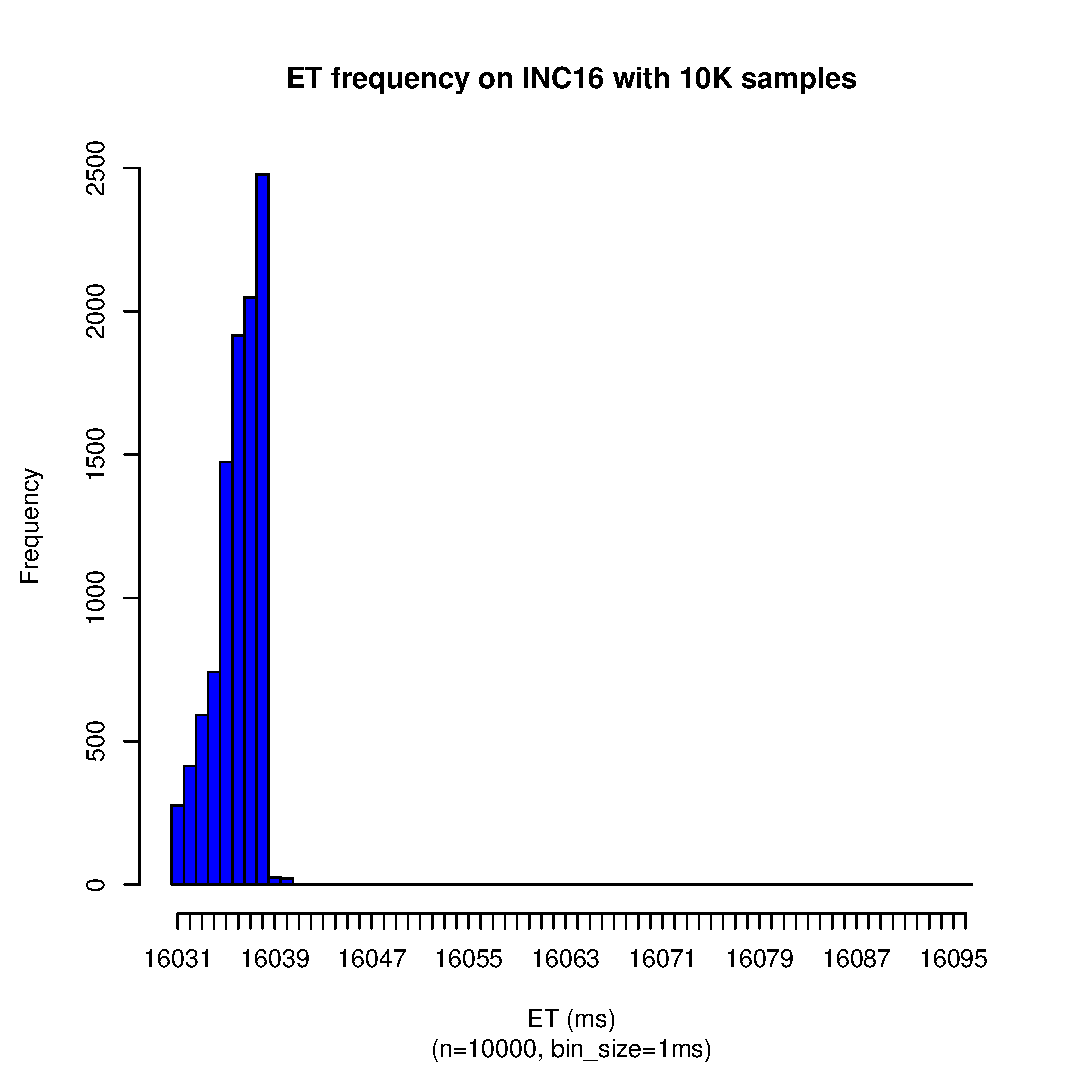
\includegraphics[scale=0.43]{10k_run/16_sec_et_hist_v5.eps}
		\label{fig:inc16_10k_et_hist_v5}
	}
	\subfigure[PT frequency on INC16]{
		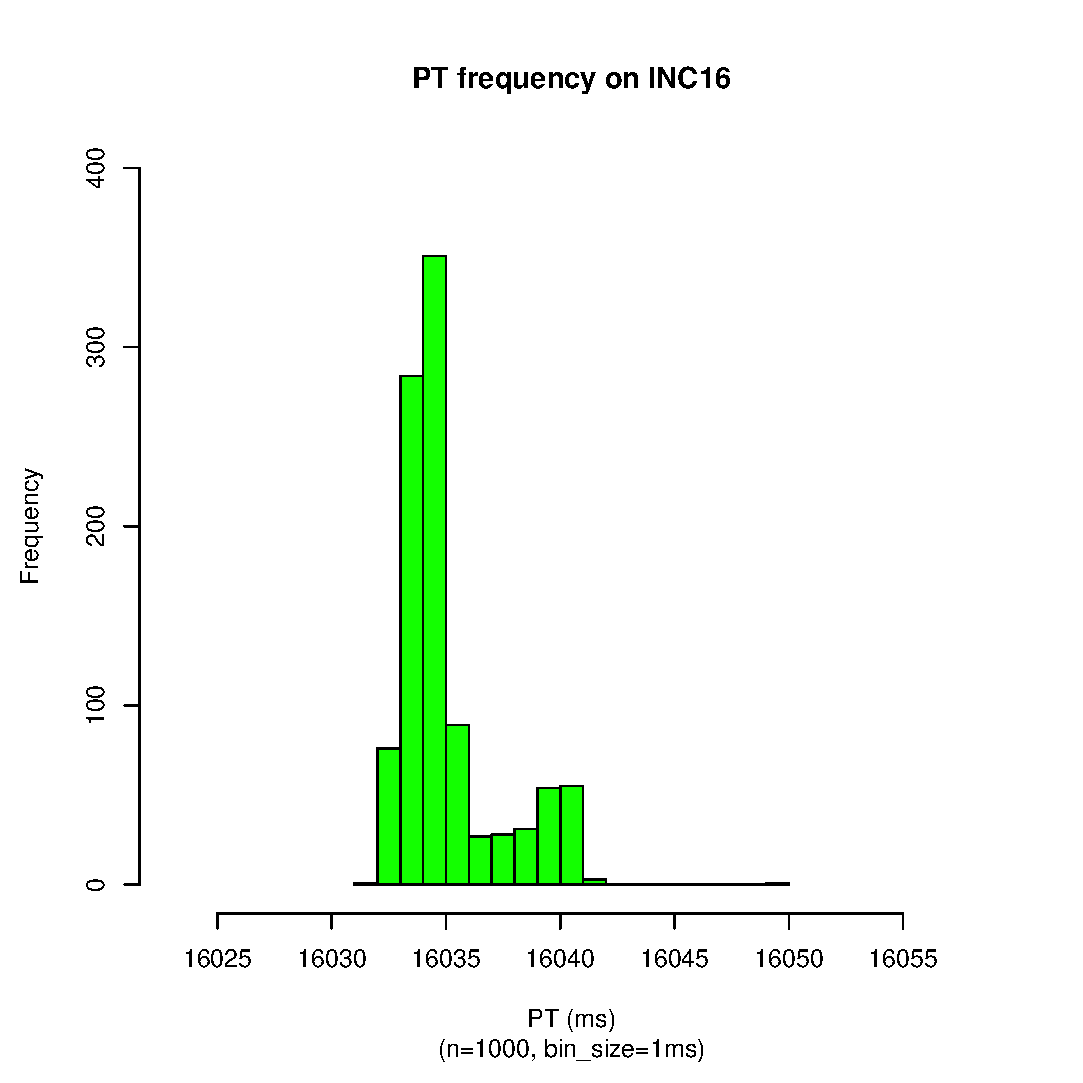
\includegraphics[scale=0.43]{10k_run/16_sec_pt_hist_v5.eps}
		\label{fig:inc16_10k_pt_hist_v5}
	}
	\caption{Histograms of INC8 and INC16 with 10,000 samples~\label{fig:10k_run_hist}}
\end{figure}
